\documentclass{report}

\usepackage{amsmath,amssymb,amsfonts}
\usepackage{algorithmic}
\usepackage{graphicx}
\usepackage{textcomp}
\usepackage{xcolor}
\usepackage{tikz}
\usepackage[version=4]{mhchem}
\usepackage{booktabs}
\usepackage{multirow}
\usepackage{siunitx}
\usepackage{eurosym}
\usepackage{mhchem}
\usepackage{amssymb}
\usepackage{amsthm}
\usepackage{tikz}
\usepackage{pgfplots}
\usepackage{multirow}
\usepackage{graphicx}
\usepackage{hyperref}
\usepackage{eurosym}
\usepackage[utf8]{inputenc} % for UTF-8 input encoding
\usepackage[T1]{fontenc}    % for correct font encoding
\usepackage{lipsum}         % for generating dummy text
% \def\BibTeX{{\rm B\kern-.05em{\sc i\kern-.025em b}\kern-.08em
%     T\kern-.1667em\lower.7ex\hbox{E}\kern-.125emX}}
\usepackage{url}

\usepackage[backend=biber, style=numeric]{biblatex} % for bibliography

\hypersetup{
    colorlinks=false,
    linkbordercolor={1 1 1}, % White {R G B}
    pdfborderstyle={/S/U/W 1} % Style of border: underline, width 1pt
}
% Define the 'definition' environment
\newtheorem{definition}{Definition}

\addbibresource{bibliography/Bibliography.bib}

\title{Bidding stochastic demand for ancillary services: the P90 rule}
\author{Peter A. Vistar Gade}
\date{\today}

\begin{document}

\maketitle

% \tableofcontents

\section*{Introduction}


\begin{figure}[!t]
    \centering
    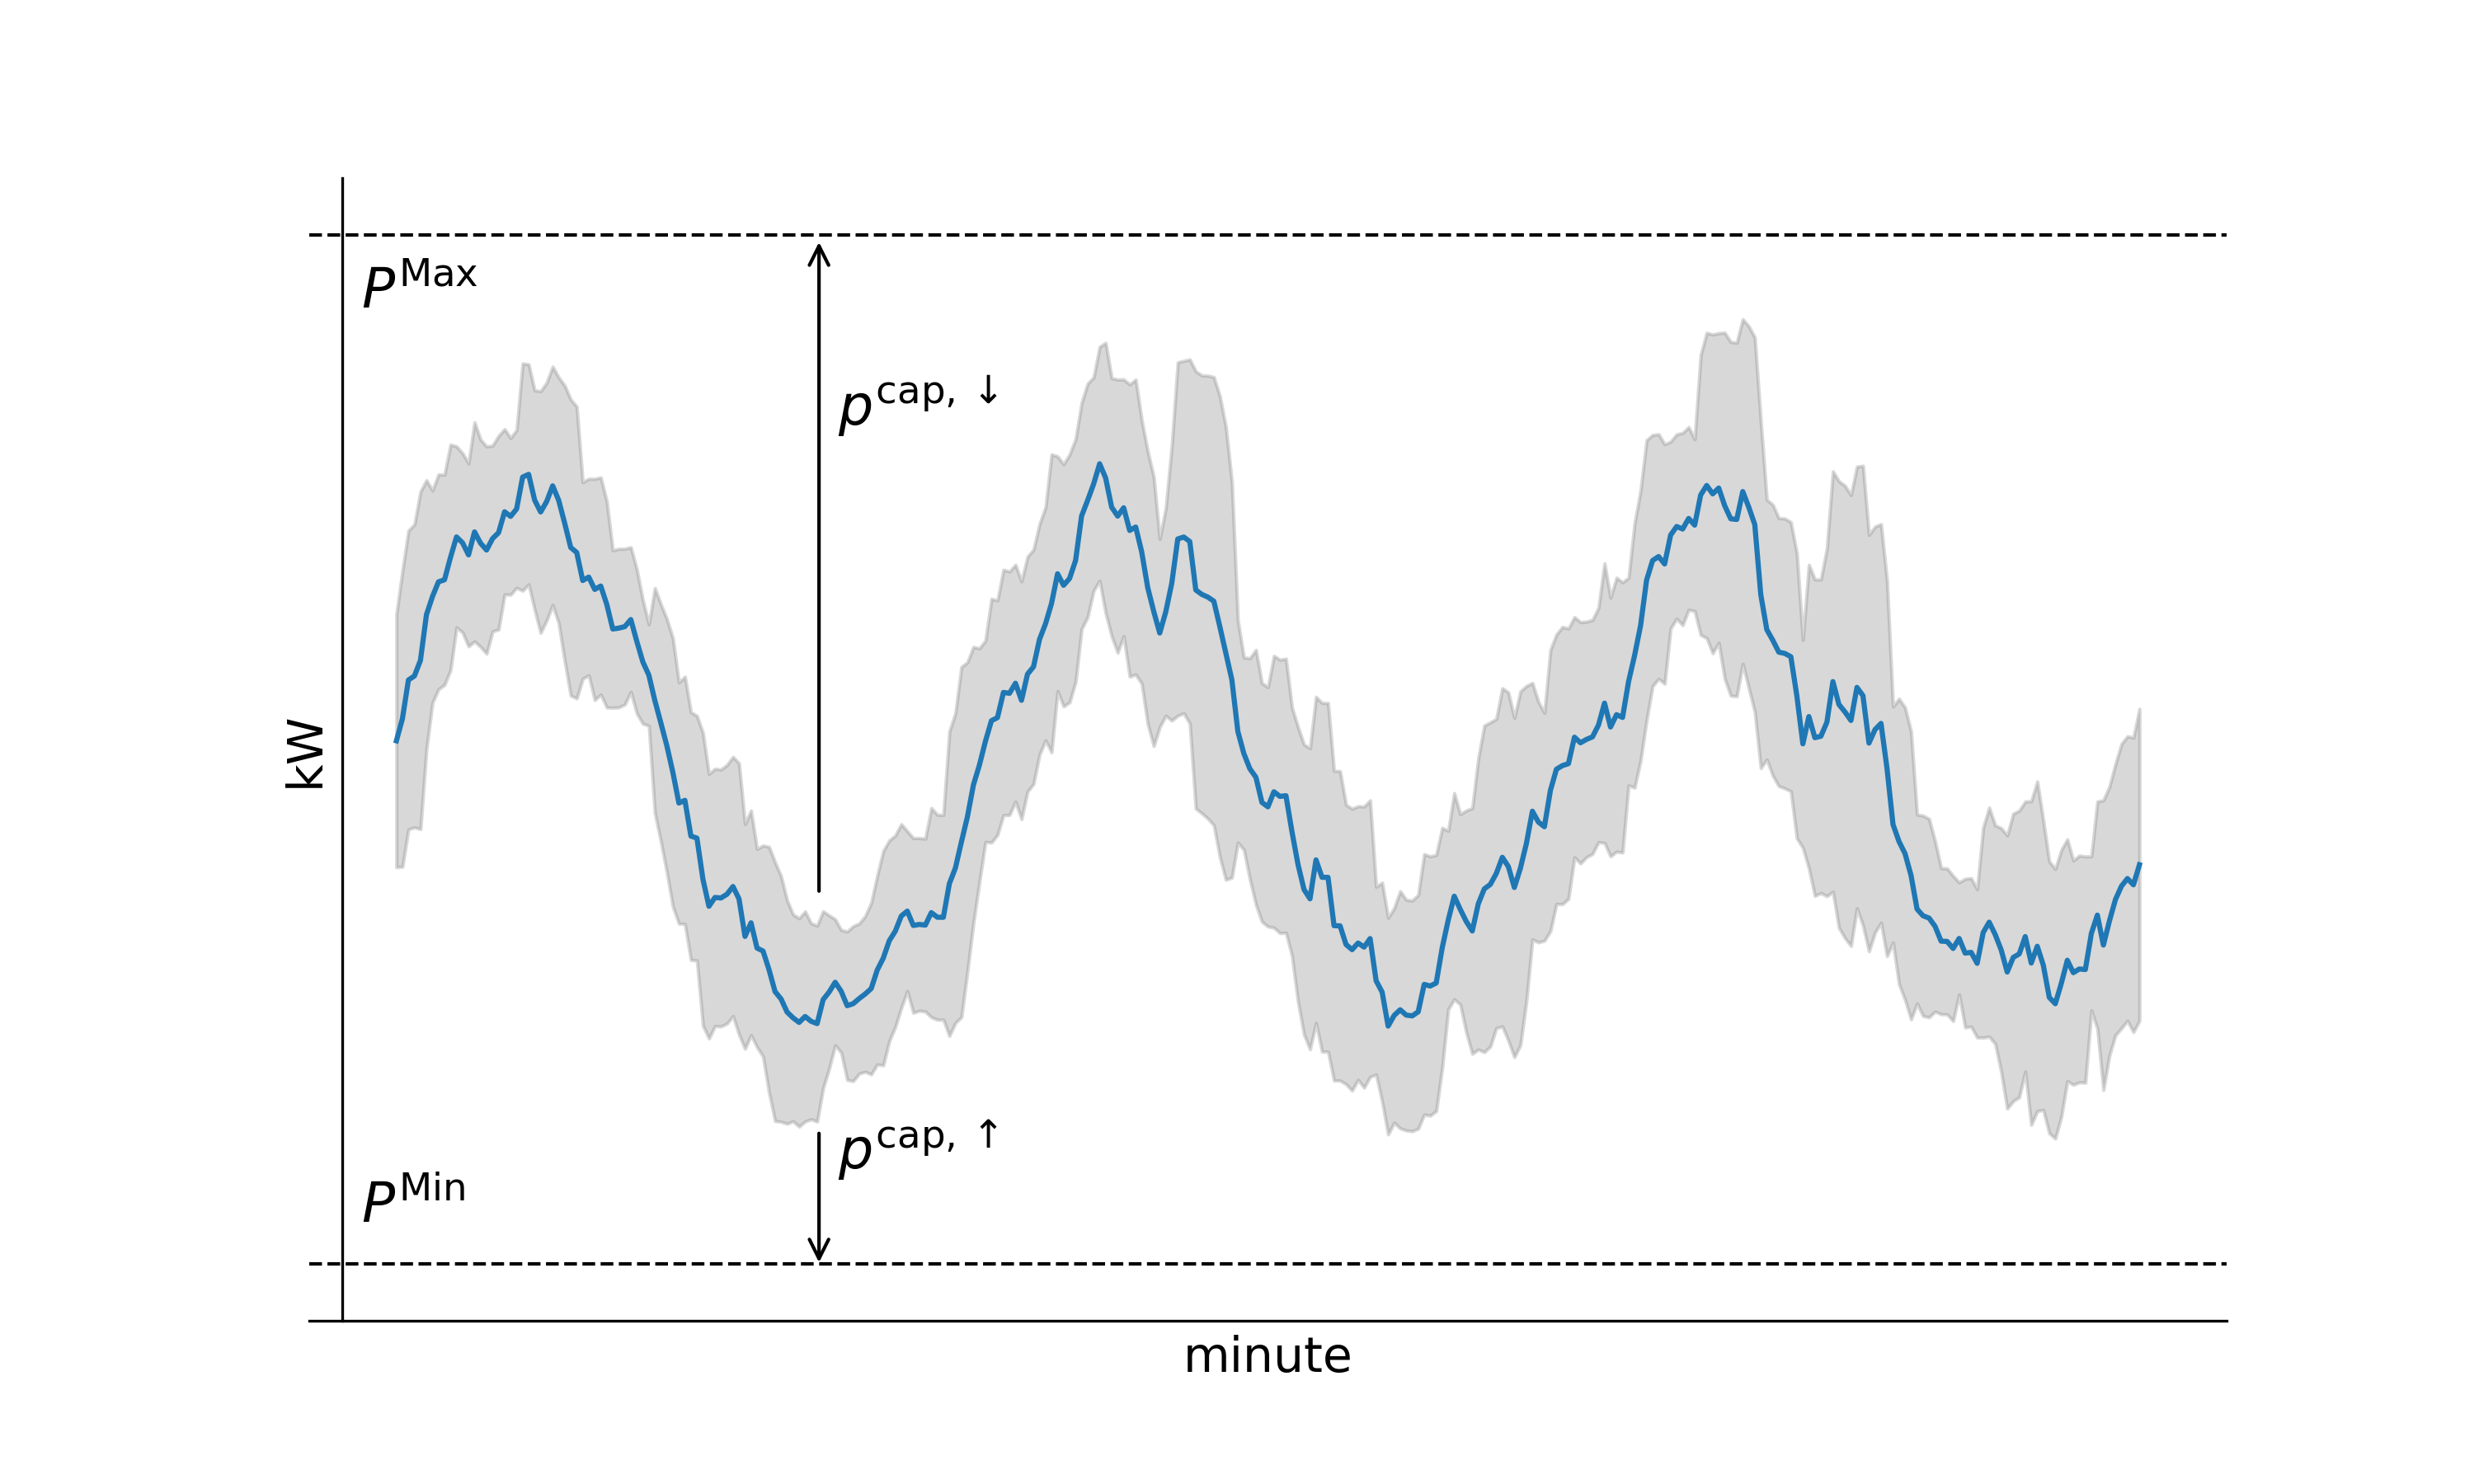
\includegraphics[width=0.99\textwidth]{figures/power_high_res_plot.png}
    \caption{Uncertain power consumption of flexible demand portfolio, denoted by $p_{m}^{\text{B}}(\xi)$. The available capacity for bidding flexibility for a given time instance is illustrated as $p^{\text{cap},\downarrow}$ for down-regulation and $p^{\text{cap},\uparrow}$ for up-regulation. $P^{\text{Max}}$ and $P^{\text{Min}}$ is the  maximum and minimum power consumption of the portfolio, respectively.}
    \label{fig:power}
\end{figure}

\noindent Abbreviations:

\begin{itemize}
    \item \textbf{C}hance \textbf{C}onstraint: \textbf{CC}
    \item \textbf{J}oint \textbf{C}hance \textbf{C}onstraint: \textbf{JCC}
    \item \textbf{D}istributionally \textbf{R}obust \textbf{J}oint \textbf{c}hance \textbf{c}onstraint: \textbf{DRJCC}
\end{itemize}

\noindent Sets:

\begin{itemize}
    \item $\mathcal{H} = \{1, 2,  \ldots 24\}$
    \item $\mathcal{M} = \{1, 2,  \ldots 1440\}$
    \item $ \mathcal{M}_{h} = \{h \times 60 + m \mid m \in \{0, 1, 2, \ldots, 59\}\}$

\end{itemize}

\noindent Definitions:

\begin{definition}[Energinet's P90 rule \cite{energinet}]
    This means, that the participant's prognosis, which must be approved by Energinet, evaluates that the probability is 10\% that the sold capacity is not available. This entails that there is a 90\% chance that the sold capacity or more is available. This is when the prognosis is assumed to be correct.

    The probability is then also 10\%, that the entire sold capacity is not available. If this were to happen, it does not entail that the sold capacity is not available at all, however just that a part of the total capacity is not available. The available part will with high probability be close to the sold capacity.
\end{definition}


\noindent Problem \ref{P1} optimizes reserve capacity for a flexible demand (Figure \ref{fig:power}) such that there is at least a $1-\epsilon$ probability of fulfilling the P90 requirement from Energinet.

\begin{align}\label{P1}
    \max_{p_{h}^{\text{cap}, \uparrow}, p_{h}^{\text{cap}, \downarrow}} \quad & \sum_h \left( \lambda_h p_{h}^{\text{cap}, ,\uparrow} + \lambda_h p_{h}^{\text{cap},\downarrow} \right)                                                                                               \\
    \text{s.t.} \quad                                                         & \mathbb{P}  \left( p_{h}^{\text{cap}, \uparrow} \leq P_{m}^{\text{B}}(\xi) - P^{\text{Min}}, \quad \forall{h} \in \mathcal{H}, \forall{m} \in \mathcal{M}_{h}  \right)   & \geq 1 - \epsilon          \\
                                                                              & \mathbb{P}  \left( p_{h}^{\text{cap}, \downarrow} \leq P^{\text{Max}} - P_{m}^{\text{B}}(\xi), \quad \forall{h} \in \mathcal{H}, \forall{m} \in \mathcal{M}_{h}  \right) & \geq 1 - \epsilon          \\
                                                                              & p_{h}^{\text{cap},(.)} \leq P^{\text{Max}},                                                                                                                              & \forall{h} \in \mathcal{H} \\
                                                                              & p_{h}^{\text{cap},(.)} \geq 0,                                                                                                                                           & \forall{h} \in \mathcal{H}
\end{align}

Here, we note that Problem \ref{P1} can be simplified by assuming symmetric flexibility, i.e., $p_{h}^{\text{cap},\downarrow} = p_{h}^{\text{cap},\uparrow} = p_{h}^{\text{cap}}$. Then the two JCCs are essentially the same since the uncertain power consumption, $P_{h}^{\text{B}}(\xi)$, is simply set to $P_{h}^{\text{B}}(\xi) \triangleq \min \{ P_{h}^{\text{B}}(\xi) - P^{\text{Min}}, P^{\text{Max}} - P_{h}^{\text{B}}(\xi) \}$.

Problem \ref{P1} can be simplified further by only considering each minute within that hour within one JCC (and omitting trivial constraints for bounding capacity for cleanness):

\begin{align}\label{P2}
    \max_{p_{h}^{\text{cap}}} \quad & \sum_h \lambda_h p_{h}^{\text{cap}}                                                                                                                             \\
    \text{s.t.} \quad               & \mathbb{P}  \left( p_{h}^{\text{cap}} \leq P_{m}^{\text{B}}(\xi), \quad \forall{m} \in \mathcal{M}_{h}  \right) \geq 1 - \epsilon, & \forall{h} \in \mathcal{H}
\end{align}

Problem \ref{P2} is now decomposed by hour and each hour can be solved in parallel to obtain $p_{h}^{\text{cap}}$, $\forall{h} \in \mathcal{H}$.

Doing so, the $h$ index can be removed and Problem \ref{P2} contains one JCC:

\begin{align}\label{P3}
    \max_{p^{\text{cap}}} \quad & \lambda p^{\text{cap}}                                                                                                             \\
    \text{s.t.} \quad           & \mathbb{P}  \left( p^{\text{cap}} \leq P_{m}^{\text{B}}(\xi), \quad \forall{m} \in \mathcal{M}_{h}  \right) \geq 1 - \epsilon &  &
\end{align}

The uncertainty, $\xi$, is seen in Figure \ref{fig:power} on the realized power consumption, $p_{m}^{\text{cap}}(\xi)$. To solve Problem \ref{P3}, we need to create a sample set  $p_{m}^{\text{cap}}(\xi)$ governed by $\mathbb{P}$ from either:

\begin{enumerate}
    \item Historical data
    \item A predictive forecast (e.g., quantile or probabilistic)
\end{enumerate}

We are interested in two methods for approximating the JCC in Problem \ref{P3}: (i) CVaR approximation and (ii) ALSO-X \cite{jiang2022also}.

\subsection*{CVaR}

\begin{align}\label{P4}
    \max_{p^{\text{cap}}} \quad & \lambda p^{\text{cap}}                                                                                                                \\
    \text{s.t.} \quad           & \mathbb{P}\text{-CVaR}_{1-\epsilon} \left( p^{\text{cap}} \leq P_{m}^{\text{B}}(\xi), \quad \forall{m} \in \mathcal{M}_{h}  \right) &
\end{align}

\subsection*{ALSO-X}

\begin{align}\label{P5}
    \max_{p^{\text{cap}}} \quad & \lambda p^{\text{cap}}                                                                                                       \\
    \text{s.t.} \quad           & \text{ALSO-X}_{1-\epsilon} \left( p^{\text{cap}} \leq P_{m}^{\text{B}}(\xi), \quad \forall{m} \in \mathcal{M}_{h}  \right) &
\end{align}

\section*{DRJCC}

In this section, we take a different approach. Converting Problem \ref{P3} to its distributionally robust counterpart, we get:

\begin{align}\label{PP1}
    \max_{p^{\text{cap}}} \quad & \lambda p^{\text{cap}}                                                                                                                                               \\
    \text{s.t.} \quad           & \min_{_{\mathbb{P} \in \mathcal{P}}}  \mathbb{P} \left( p^{\text{cap}} \leq P_{m}^{\text{B}}(\xi), \quad \forall{m} \in \mathcal{M}_{h}  \right) \geq 1 - \epsilon &
\end{align}

It is still possible to use CVaR and ALSO-X for Problem \ref{PP1} as it yields tractable, linear formulations \cite{ordoudis2021energy} for CVaR and ALSO-X \cite{jiang2023also}.

\section*{Number of samples required}

\printbibliography

\end{document}
